% TexPage：XeLaTeX，TeX Live 2025 或更新；本文件与两个 PDF 图片放在同一目录。
\documentclass[UTF8,fontset=fandol,a4paper,zihao=-4]{ctexart}
\usepackage[margin=2.4cm]{geometry}
\usepackage{lmodern,amsmath,booktabs,array,graphicx}
\usepackage{xcolor}
\usepackage[colorlinks=true,linkcolor=blue!60!black,urlcolor=blue!60!black,citecolor=blue!60!black]{hyperref}

\newcommand{\StudentName}{樊沛山}
\newcommand{\StudentID}{2026018108}
\newcommand{\StudentUnit}{人工智能学院}
\hypersetup{pdftitle={共享单车的周末使用节律差异},pdfauthor={\StudentName}}
\setlength{\emergencystretch}{2em}
\linespread{1.15}
\pagestyle{plain}
\renewcommand{\arraystretch}{1.18}
\urlstyle{same}
\title{共享单车的周末使用节律差异\\[0.4em]
  \large 基于 Divvy 与 NOAA 数据的探索和跨年验证}
\author{\StudentName\quad 学号：\StudentID\\\StudentUnit\\“人工智能与科学研究”课程 · Vibe Coding 作业}
\date{} % 封面不显示日期。

\begin{document}
\maketitle

\begin{abstract}
利用 AI 辅助编程，对芝加哥 Divvy 行程与 NOAA 日天气开展质量诊断、描述统计、时空可视化和天气关联分析。2024 年发现非会员的周末/平日日均行程比高于会员，据此提出明确假设，并在运行前固定 2025 年验证规则。验证年会员比值为 0.733，非会员为 1.519，两组比值之比 $Q=2.071$，95\% 近似周块稳定性区间为 $[1.985,2.164]$，满足预设初步支持判据。额外按月份、10\,$^\circ$C 气温区间与降水状态分层，27 个共同支持格覆盖 221 天，日期加权几何汇总 $Q=1.983$，方向一致。结论限于既定筛选口径及共同支持范围，不作因果解释。报告分别记录 AI 辅助发现与研究者的选题和规则判断。
\end{abstract}

\section{研究问题与证据划分}

课程提供数据而不预先指定问题。本研究关注两种行程标签的周末节律差异：\textbf{非会员的周末/平日日均行程比是否高于会员？}这里 member/casual 是行程上的来源标签，不能据此计算独立用户数或识别出行动机。

会员与非会员的总规模不同，平日与周末的天数也不同，因此先比较每组两类日期的日均量，再比较两组的比值。研究划分三层证据：2024 年用于发现线索，2025 年全年用于主验证，2025 年月份与天气分层用于额外稳健性描述。全历史用于归档和质量覆盖检查，不直接混合疫情、系统扩张及字段变化时期研究行为规律。

发现/验证年份在行为及天气关联探索前确认。整理阶段已知各年的覆盖与清洗计数，但未用 2025 年关系结果选择问题或分箱。主指标、重抽样和额外实验规则先保存并经审阅，再执行验证\cite{repo}。

\section{数据来源与整理}

\subsection{下载范围与分析范围}

使用 Divvy 官方历史行程\cite{divvy}，并下载 NOAA GHCN-Daily 两个站点的完整档案\cite{noaa}。主分析使用 Chicago O'Hare（USW00094846），Midway（USW00014819）仅作备用资料保存，未跨站填补。行程按本地出发日期与天气日期标签连接。

截至 2026-11-09，归档 97 个行程 ZIP，覆盖 2013-06-27 至 2026-10-31，共含 109 个行程 CSV；全部来源归档文件共 110 个、1.829 GiB。逐文件记录来源、下载时间、大小与 SHA-256，并检查压缩包完整性。全量标准化表有 58,978,535 行，筛选后有 49,227,733 行。

\begin{center}
\begin{tabular}{lrrr}
\toprule
范围 & 原始行程 & 筛选行程 & 用途\\
\midrule
2024 年 & 5,860,621 & 4,121,607 & 发现，366 天\\
2025 年 & 5,552,964 & 3,661,513 & 验证，365 天\\
\bottomrule
\end{tabular}
\end{center}

天气包含 PRCP、SNWD、SNOW、AWND、TMAX、TMIN。PRCP 由 0.1 mm 转为 mm，SNWD/SNOW 保持 mm；AWND 由 0.1 m/s 转为 m/s，温度由 0.1\,$^\circ$C 转为\,$^\circ$C。原值、转换值、质量标记与可用值分开保留；缺失不补零，T 微量标记保留。2024 年探索变量及 2025 年分层所需温度、降水均无缺失。

历史站点资料与当前 GBFS 分开保存；当前快照有 2,079 个站点，不用于回填过去的行程。2013 年和 2026 年不是完整年度。

\subsection{筛选规则及数量变化}

全量表保留全部原始行与追溯字段；分析使用另存的筛选子集。规则由研究者在对话中确认，按表中顺序执行。

\begin{center}
\small
\begin{tabular}{p{0.43\linewidth}rr}
\toprule
规则 & 本步移除 & 本步保留\\
\midrule
行程 ID 完整 & 0 & 58,978,535\\
起止时间可解析 & 0 & 58,978,535\\
时长在 [60, 86400] 秒，含边界 & 883,535 & 58,095,000\\
起终点 ID、名称四项完整 & 8,820,241 & 49,274,759\\
同 ID 完全相同记录仅保留一条 & 80 & 49,274,679\\
排除明确标注的 electric\_scooter & 46,946 & 49,227,733\\
\bottomrule
\end{tabular}
\end{center}

同 ID 但内容冲突的记录保留并标记，仍须满足其余规则；旧版与新版 ID 分属两个命名空间。旧数据优先用原报秒数，避免分钟精度时间戳造成取整差异；车型未提供的历史记录保留。时间沿用本地墙上时间，不擅自转换为 UTC，夏令时附近仍可能有歧义。

筛选会改变样本构成。2024 年在满足其他规则的记录中，普通自行车的站点信息完整率为 99.998\%，电动自行车仅为 49.04\%；会员和非会员对应为 73.65\% 和 74.10\%。两种用户标签的总体比例接近，仍不能排除条件性的选择偏差，故结论针对通过筛选的行程。

\section{2024 年的四类探索}

探索通过根目录 uv 环境运行，输出 6 组 PNG/PDF 图和 14 份 CSV 汇总。所有行为与天气关系统计限定在 2024 年；每组每天最多一个天气关联观测。

\begin{center}
\small
\begin{tabular}{p{0.17\linewidth}p{0.73\linewidth}}
\toprule
类别 & 主要内容和发现\\
\midrule
质量诊断 & 检查全历史覆盖与保留率，比较站点完整性在车型和用户标签间的差异；历史保留率也受发布口径影响。\\
描述统计 & 统计行程数、时长、同站返回和周末/平日差异；非会员的时长中位数更高。\\
时空可视化 & 绘制月度、小时与站点空间分布；非会员和会员的时间节律不同，站点 ID 存在名称变体。\\
天气关联 & 比较气温、降水、风速、降雪与日行程量的原始及分层指数关联，识别季节混杂。\\
\bottomrule
\end{tabular}
\end{center}

\subsection{用户标签、时间与空间差异}

2024 年会员有 2,640,636 条行程，非会员有 1,480,971 条。两组时长中位数分别为 8.92、13.70 分钟，第 95 百分位分别为 32.86、74.30 分钟；同站 ID 起终比例为 2.44\%、8.66\%。逐日比较中，349/366 天的非会员中位时长更长，日中位时长差的中位数为 3.31 分钟。

会员的周末/平日日均量比为 0.770，非会员为 1.580，12 个月均是非会员更高，形成后续研究线索（图~\ref{fig:discovery}）。平日预设早晚六小时（7—9 时、16—18 时）的行程份额为会员 50.4\%、非会员 40.7\%，但不能据此判定个人出行目的。

全年有 1,717 个出发站点 ID，前 10 个贡献筛选行程的 8.67\%；85 个 ID 对应多个站名。空间图使用当年行程坐标的中位点，不按名称自动合并，也不用当前站点反推历史。

\subsection{天气关联与季节混杂}

以当日行程数除以本组同月、同日类型的均值，乘以 100，构造描述性分层指数。气温中点与原始日行程量的 Spearman 相关为会员 0.82、非会员 0.87；指数归一化后降为 0.15、0.23，提示原始强关联混合了季节差异。温度中点 $(T_{\max}+T_{\min})/2$ 不是实测日均温。

2024 年有 196 个无雨日、75 个微量/不足 1 mm 日、95 个至少 1 mm 雨日。雨日/无雨日的平均分层指数比为会员 0.831、非会员 0.760；但分层后的降水秩相关分别为 $-0.32$、$-0.31$，相近且未充分控制温度。这些数字只是候选线索，不是已证实的组间降水效应。

\section{问题发现与假设}

AI 根据上述探索提出三个候选：A，周末/平日比的组间差异；B，同一天的行程中位时长差异；C，雨日相对行程量降低的组间差异。研究者选择 A，并将天气分层作为额外实验。B、C 未进入验证。

令 $Y_{g,d}$ 为日期 $d$、标签 $g$ 的筛选行程数，$E$ 为周末日期集，$W$ 为平日日期集。定义
\begin{equation}
 R_g=\frac{\sum_{d\in E}Y_{g,d}/|E|}{\sum_{d\in W}Y_{g,d}/|W|},
 \qquad Q=\frac{R_{\mathrm{casual}}}{R_{\mathrm{member}}}.
\end{equation}
原假设 $H_0:Q\leq 1$，研究假设 $H_1:Q>1$。$Q$ 比较两组各自的周末/平日比，不等于两组周末行程量之比，也不要求非会员每个月的 $R$ 都大于 1。

\begin{figure}[htbp]
 \centering
 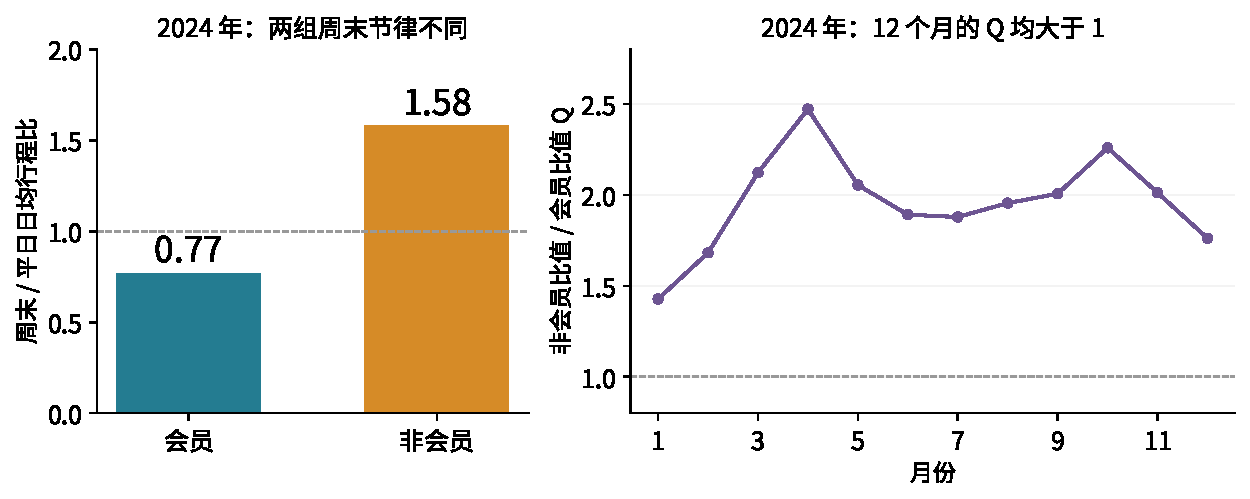
\includegraphics[width=\linewidth]{discovery.pdf}
 \caption{2024 年发现。非会员的周末/平日比为 1.580，会员为 0.770；12 个月的比值之比均大于 1。发现年结果用于提出问题，不作确认性检验。}
 \label{fig:discovery}
\end{figure}

\section{预设验证方法}

\subsection{2025 年全年主验证}

固定范围为 2025-01-01 至 2025-12-31。周六、日为周末，其余为平日，不重新标记节假日。日历有 104 个周末日、261 个平日。两组用同一批日期；全量来源当天有记录而某组无筛选行程时记为零，来源整日未观测时暂停核查，不能记为零。两种标签$\times$两种日类型的四个总量有零时，不加伪计数，报告主指标不可估。

按自然周配对重抽样，同一周内两组、日期标签和行程数一起抽取，保留部分相邻日期结构。以周一日期作为周键，年首尾不完整周保留。每块按首个实际观测日的月份归层，各月有放回抽取原块数，共 10,000 次，随机种子为 20261109。每次重新计算 $Q$，取第 2.5\%、97.5\% 分位，形成近似稳定性区间；有效抽样不足 99\% 时不作主判定。

时间序列重抽样需考虑相关性\cite{bootstrap}。本方案采用自然周和月份的近似设计，并非文献所述 STL 残差重抽样算法。它依赖同月周块近似可交换的假设，月份构成也仅近似保留，不能完全处理更长的时间相关性。

预设判据为 $Q>1$ 且区间下界大于 1 时获得初步支持；$Q>1$ 但下界不超过 1 时仅方向一致、证据不足；$Q\leq 1$ 时不支持预期方向。主判据不因月度或额外实验结果而切换，不按数百万条行程独立检验并报告 p 值。

\subsection{额外实验：月份与天气共同支持}

仅用 2024 年天气与日期比较设计覆盖：在每格至少两种日类型各 2 天时，5\,$^\circ$C 分箱覆盖 144/366 天、11 个月，10\,$^\circ$C 分箱覆盖 226/366 天、12 个月。研究者选择后者，选择过程未按行程效应筛选。

2025 年采用月份$\times$10\,$^\circ$C 气温区间$\times$三类降水。温度中点以 0\,$^\circ$C 为原点，区间左闭右开，例如 $-1\,{}^\circ\mathrm{C}\in[-10,0)$。降水定义为：
\begin{center}
\begin{tabular}{ll}
\toprule
状态 & 判定\\
\midrule
无雨 & PRCP=0 且没有 T 微量标记\\
微量/不足 1 mm & 有微量标记的零值，或 $0<\mathrm{PRCP}<1$ mm\\
至少 1 mm & $\mathrm{PRCP}\geq1$ mm\\
\bottomrule
\end{tabular}
\end{center}

同格至少有 2 个周末日、2 个平日才纳入共同支持。规则只使用日期与天气；缺失或不可用天气只从额外实验排除，不影响全年主分析。对每个支持格 $s$ 计算 $Q_s$，以日期数 $n_s$ 加权：
\begin{equation}
 Q_{\mathrm{strat}}=\exp\!\left(\sum_s w_s\log Q_s\right),
 \qquad w_s=\frac{n_s}{\sum_s n_s}.
\end{equation}
至少有 5 个支持格才报告该汇总；若任一支持格的四个总量有零，则保留原格和计数，但总体对数汇总不可估，不临时剔格或加伪计数。额外实验不另作显著性检验，只报告方向及覆盖；不根据验证年结果放宽阈值。

\section{验证结果}

\subsection{全年比值及稳定性}

2025 年筛选行程均属于 member/casual，来源日期无整日缺失。两组日均量及比值如下。

\begin{center}
\begin{tabular}{lrrr}
\toprule
标签 & 平日日均量 & 周末日均量 & $R_g$\\
\midrule
会员 & 6,971.98 & 5,113.16 & 0.733\\
非会员 & 3,127.11 & 4,748.86 & 1.519\\
\bottomrule
\end{tabular}
\end{center}

比值之比 $Q=2.071$。53 个周块的 10,000 次重抽样全部有效，95\% 近似稳定性区间为 $[1.985,2.164]$，下界大于 1，满足预设初步支持判据。2024 年发现值约为 2.053，跨年方向一致，但发现值不作为新增验证结果。

2025 年 12 个月的 $Q$ 均大于 1，最小为 1 月的 1.479，最大为 10 月的 2.200；它们是异质性描述，未另外检验各月显著性。非会员自身 1、2 月的 $R$ 仍低于 1，符合前述相对组间假设的定义。

\subsection{天气分层及共同支持范围}

2025 年有 80 个非空格，其中 27 格满足支持条件，覆盖 221/365 天（60.5\%），包括 148 个平日和 73 个周末日，涉及全部 12 个月。无天气缺失排除日，其余 144 天因同格两种日类型支持不足排除。全年主分析仍保留 365 天。

\begin{center}
\small
\begin{tabular}{p{0.43\linewidth}rr>{\raggedright\arraybackslash}p{0.23\linewidth}}
\toprule
比较 & 天数 & $Q$ & 不确定性处理\\
\midrule
全年未分层 & 365 & 2.071 & 近似稳定性区间 $[1.985,2.164]$\\
共同支持日期，未分层 & 221 & 1.981 & 描述性点估计\\
同批日期，分层汇总 & 221 & 1.983 & 日期加权几何平均，描述性\\
\bottomrule
\end{tabular}
\end{center}

27 个支持格的 $Q_s$ 均大于 1，且四个总量均为正，无须触发不可估规则。共同支持范围内的分层结果方向一致，为主结果提供方向性稳健性证据，但不能将逐格同向解释为逐格显著。全年与共同支持结果见图~\ref{fig:validation}。

\begin{figure}[htbp]
 \centering
 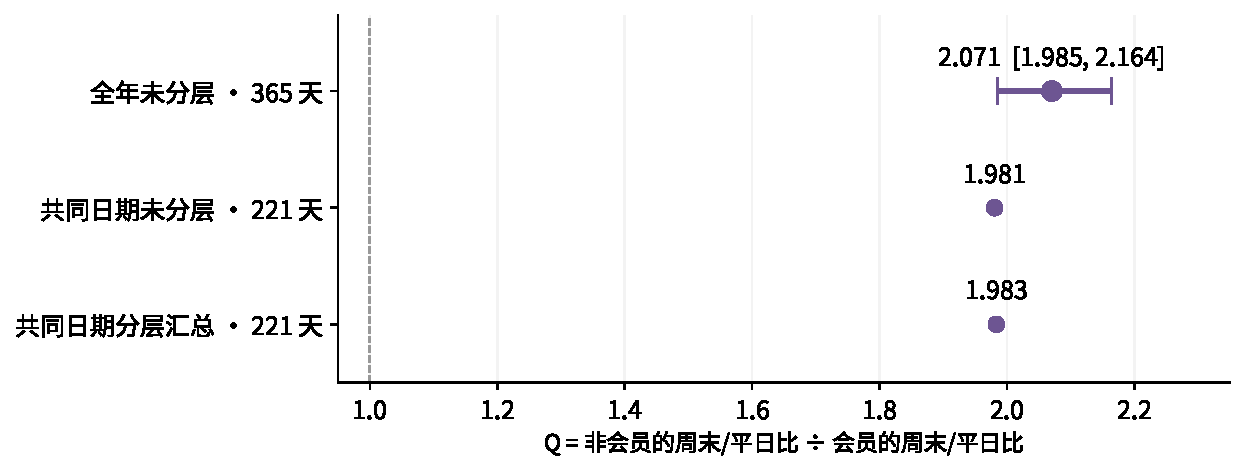
\includegraphics[width=\linewidth]{validation.pdf}
 \caption{2025 年主验证及额外实验。仅全年点附 95\% 近似周块稳定性区间；共同支持两项仅作描述。分层汇总为日期加权几何平均，覆盖 27 格、221 天。三项的日期范围或统计目标不同。}
 \label{fig:validation}
\end{figure}

全年与共同日期的比较改变了日期范围；共同日期内的分层汇总又改变了汇总方式及统计目标。因此不使用这些数值差异计算“天气解释了多少差异”，也不将 221 天内的结论直接推广至其余日期。

\section{讨论与局限}

两种标签的相对节律差异在 2025 年复现，在天气共同支持范围内保持方向一致。主要限制为：
\begin{enumerate}
 \item \textbf{样本选择。}站点信息完整性筛选显著改变车型构成；用户标签总体完整率接近不能消除条件选择偏差。
 \item \textbf{时间与日历。}周块区间是近似稳定性描述；节假日、跨月周、季节和运营变化仍可能影响结果。2024、2025 年也不代表完全独立的个人样本。
 \item \textbf{天气与支持。}机场单站只代理城市天气，10\,$^\circ$C 格内仍可能有温度差异；额外实验仅覆盖全年 60.5\% 日期。
 \item \textbf{解释范围。}没有独立用户身份及出行目的，不能判断个人通勤、旅游或因果效应。观察到的标签节律不能解释为改变会员身份会改变行为。
\end{enumerate}

\section{AI 使用与研究者判断}

\begin{center}
\small
\begin{tabular}{p{0.43\linewidth}p{0.47\linewidth}}
\toprule
AI 辅助工作 & 研究者实际作出的判断\\
\midrule
阅读任务，提出分阶段流程 & 确认全部历史下载、中文短汇报和 Beamer 格式\\
编写下载、整理、分析和测试程序 & 确认时长、站点完整性、重复和车型筛选规则\\
归纳 2024 年模式，提出 A/B/C & 选择 A；确认 2024 发现、2025 验证\\
比较天气分层覆盖，拟定具体验证方法 & 选择细分层与 10\,$^\circ$C；通过 PR 审阅规则及实现\\
执行计算、制图、整理报告与汇报 & 审阅阶段 PR，删改报告与汇报表述\\
\bottomrule
\end{tabular}
\end{center}

统计线索、候选问题和计算结果记录为 AI 辅助产生，不记作研究者独立发现。下载脚本曾根据 PR 自动 review 修复缓存清单保留问题，反映 AI 产物仍须检查。用户通过逐阶段 PR 审阅监督文件修改；核心假设与规则的来源记录在仓库研究日志。

\section{复现}

项目统一使用根目录 uv 和 \path{.venv/}，依赖由 \path{uv.lock} 固定。Python 代码、来源清单、配置、聚合结果及运行记录见仓库\cite{repo}；原始数据和大表保存在服务器。已有原始与整理数据时，可从对应后续步骤运行，完整流程为：

\begin{quote}\small\ttfamily
uv sync --locked\\
uv run python -m scripts.download\_data\\
uv run python -m scripts.verify\_data\\
uv run python -m scripts.prepare\_data\\
uv run python -m scripts.explore\_data\\
uv run python -m scripts.check\_weekend\_plan\\
uv run python -m scripts.validate\_weekend\\
uv run python -m scripts.prepare\_deliverables\\
uv run python -m unittest discover -s tests -v
\end{quote}

重新下载时官方可获取月份可能增加；本报告对应 2026-11-09 快照，精确版本依据来源、整理与分析清单。验证程序核对冻结配置、全部整理文件的大小及 SHA-256，检查全年计数守恒。运行记录保存代码、依赖、输入和输出校验值。

已有 27 项测试通过，包括年份边界、缺失日与零计数、配对及按月周块重抽样、日期权重和零总量支持格处理。另用独立 SQL 核对日均比值与分层汇总，并将部分重抽样逐日展开核对。汇报图从已校验汇总重绘，不增加统计分析。

\section{结论}

2025 年非会员的周末/平日日均行程比约为会员的 2.07 倍，预设周块稳定性区间下界大于 1，假设获得初步支持。月份与天气共同支持日期内的分层汇总仍大于 1，方向一致。结论限于筛选行程、近似重抽样假设及相应日期范围。

\begin{thebibliography}{9}
\small
\raggedright
\bibitem{divvy} Divvy. System Data. 数据快照：2026-11-09. \url{https://divvybikes.com/system-data}.
\bibitem{noaa} NOAA NCEI. GHCN-Daily station files and format documentation. \url{https://www.ncei.noaa.gov/pub/data/ghcn/daily/}.
\bibitem{bootstrap} Hyndman R J, Athanasopoulos G. Forecasting: Principles and Practice, 3rd ed., Section 12.5. \url{https://otexts.com/fpp3/advanced.html#bootstrapping-time-series}.
\bibitem{repo} 本研究代码、配置、聚合结果及交付材料. \url{https://github.com/AlphaSpire8/vibe_coding_homework}.
\end{thebibliography}

\end{document}
